\chapter{Evaluation}

This section is focused on the empirical evaluation of \textsc{Carico} as a
Kubernetes scheduler, comparing it against the default industry-standard
\texttt{kube-schedulers}. I was unable to compare \textsc{Carico} against any
similar telemetric-only schedulers due to their limited number and time
constraints. For the evaluation, I use a set of common scheduling objectives
used by datacenter providers~\cite{thesis}:

\textbf{Job Completion - Section \ref{sec:eval-job-completion}:}\\
Schedulers often aim to reduce the time it takes for a job or a set of jobs to
complete. In Kubernetes, Jobs are specified by a template of the Pods to be
executed, the total number of Pods to complete (\texttt{completions}) and the
maximum number of Pods running at once (\texttt{parallelism}). Job completion
is defined as the time between a Job object being published to the Kubernetes
API and the time when the last Pod of the Job completes. During the
experiments, I set \texttt{parallelism} to \texttt{completions} so that only
\texttt{kube-scheduler}'s decisions impact Job completion.

\textbf{Pod Completion - Section~\ref{sec:eval-pod-completion}:}\\
The goal of many datacenter schedulers is to complete jobs as fast as possible
so that resources are freed for subsequent jobs. For this section, I
investigate the distribution of Pod Completion, the time it takes from when a
Pod starts running to when it completes. In addition, I explain my findings
using traces of the number of concurrent Pods on each Node during job
execution.

\textbf{Resource Utilisation - Section~\ref{sec:eval-util}:}\\
Since resources are expensive, datacenters aim to ensure that resources are
well utilised with efficient placements. Over-utilisation can result in large
amounts of resource thrashing, which wastes resources and hurts a datacenters
proffitability. As \textsc{Carico} currently only uses CPU and memory metrics
for scheduling, I only measured the utilisation of those resources during the
exection of Jobs.

\textbf{Workload Heterogeneity - Section~\ref{sec:eval-hetero}:}\\
As outlined in \ref{sec:background-datacenters}, datacenters must handle
workloads with different characteristics, such as, resource usage and running
times. In this section, I evaluate how well \textsc{Carico} is able to handle
mutliple Jobs with different characteristics.

\textbf{Workload Isolation - Section~\ref{sec:eval-isolation}:}\\
Datacenters have to deal with jobs with different QoS requirements. One of
these requirements is workload isolation: the execution of one Job will not
interfere with the execution of another. With this property, users can be
guaranteed a minimum level of quality.

\textbf{Overhead - Section~\ref{sec:eval-overhead}:}\\
Due to the limited number of resources that need to be shared between users,
datacenter providers aim to mitigate the overhead from scheduling. A lower
overhead means more resources are available for users and providers can achieve
higher profits margins. For this experiment, I measure the overhead incurred
from running the DaemonSet of \textsc{Carico} Pods.

To ensure a fair comparison between \textsc{Carico} (telemetric-only scheduler)
and \texttt{kube-scheduler} (resource description-based scheduler), I use a
range of resource requests with \texttt{kube-scheduler} to highlight how much
the performance can vary with different resource request.

\section{Evaluation Setup}
These experiments ran on a Kubernetes cluster containing 20 virtual machines
(VMs) running on the Xen hypervisor. One of the machines is used as the master
Node, and the rest are worker Nodes. The master Node contains all the Pods in
the control plane, and during the evaluation of \textsc{Carico}, it contains the \textsc{Carico}
Scheduler and Aggregation Server. Each VM features four Intel Xeon Gold 6142
CPUs \@ 2.60Ghz with 8 GB of RAM running Ubuntu 24.04.2 LTS. Each CPU has a
single core with hyperthreading disabled. When running \texttt{kubectl describe
nodes}, each Node advertises $4000$ milli-CPU seconds and 8GB of RAM.

During the evaluation, I use a Prometheus deployment \cite{} to collect various
statistics, such as running Pod count, resource utilisation and Kubernetes
object completions.

%
% For any practical projects, you should almost certainly have some kind
% of evaluation, and it's often useful to separate this out into its own
% chapter.

\section{Experimental Workloads}
During the experiments I used very short-lived workloads; workloads that take
less than a minute to complete. While datacenters can expect to receive
longer-running workloads, using them in the evaluation was not feasilble due to
limited time and the need to run experiments multiple times. Short-lived tasks
can still provide valuable insights into the performance of a scheduler. Due
to their short completion time, the cost of poor scheduling decisions becomes
more significant and easier to observe.

During this evaluation, I used two types of workloads:
\begin{enumerate}
    \item \texttt{pi-2000}: A short-lived CPU-focused workload where a Pod
        computes the value of $\pi$ to 2000 decimal points.
    \item \texttt{sklearn}: A longer-running workload with a larger memory
        footprint. This Pod executes a script which uses
        \texttt{sklearn} which trains a small neural network classifier ($512$
        features, $16$ classes, $8$ hidden layers each containing $1024$
        neurons) on 5000 randomly generated samples before running inference on
        another set of 5000 randomly generated samples.
\end{enumerate}
Investigating metrics when running \texttt{pi-2000} and \texttt{sklearn} Jobs
separately demonstrates how \textsc{Carico} handles opposing resource usage
characteristics (CPU-focused vs memory-focused). Furthermore, when executing
both these Jobs concurrently, the difference in runtime helps investigate how
\textsc{Carico} also handles workloads with differnt running times.

In this experiment, I use a Job that specifies Pods that performed a small ML
workload. This workload uses a significant amount of memory, which unlike CPU,
must be carefully handled. If we increase the number of processes on a
fully-utilised CPU, it only results in each process having a smaller portion of
CPU time and degrading its performance. On the other hand, memory is less
forgiving as once memory runs out, the kernel begins OOM killing processes. This
be detrimental to Job Completion, as terminated Pods results in wasted
computations.


\section{Job Completion}
\label{sec:eval-job-completion}

% \begin{table}[ht!]
% \centering
    % \begin{tabular}{|l|r|c|c|c|c|c|}
    % \hline
    % \textbf{Scheduler} & \textbf{Requested} & \multicolumn{5}{c|}{\textbf{Job Completion (s)}} \\
    % \cline{2-7}
    % &  \textbf{CPU} & \textbf{100 Pods} & \textbf{250 Pods} & \textbf{500 Pods} & \textbf{750 Pods} & \textbf{1000 Pods} \\
    % \hline
    % Default & 100m & 15.7 $\pm$ 0.6 & 31.7 $\pm$ 2.1 & 56 $\pm$ 1.7 & 84.7 $\pm$
        % 0.6 & 112 $\pm$ 0.0 \\
    % Default & 200m & 15.7 $\pm$ 0.7 & 30.7 $\pm$ 0.6 & 55 $\pm$ 1 & 79 $\pm$ 0.0
        % & 103 $\pm$ 1 \\
    % Default & 500m & 15.7 $\pm$ 1.2 & 32 $\pm$ 2.6 & 57.7 $\pm$ 0.6 & 81 $\pm$ 2
        % & 104 $\pm$ 2.1 \\
    % Default & 1000m & 21 $\pm$ 2.0 & 54.7 $\pm$ 0.6 & 96 $\pm$ 2.6 & 133 $\pm$
        % 0.6 & 175 $\pm$ 1 \\
    % \textsc{Carico} &  & 20.3 $\pm$ 0.6 & 35.3 $\pm$ 0.6 & 60.3 $\pm$ 2.5 & 89 $\pm$ 2 &
        % 109$\pm$ 1 \\
    % \hline
    % \end{tabular}
    % \caption{Job Completion of Job deployments with different Pod counts. Each
    % Pod executed \texttt{bpi(2000)}. For the default scheduler, the requested
    % resources are also given}
    % \label{tab:pi-2000-throughput}
% \end{table}
%

\begin{figure}[ht!]
    \centering
    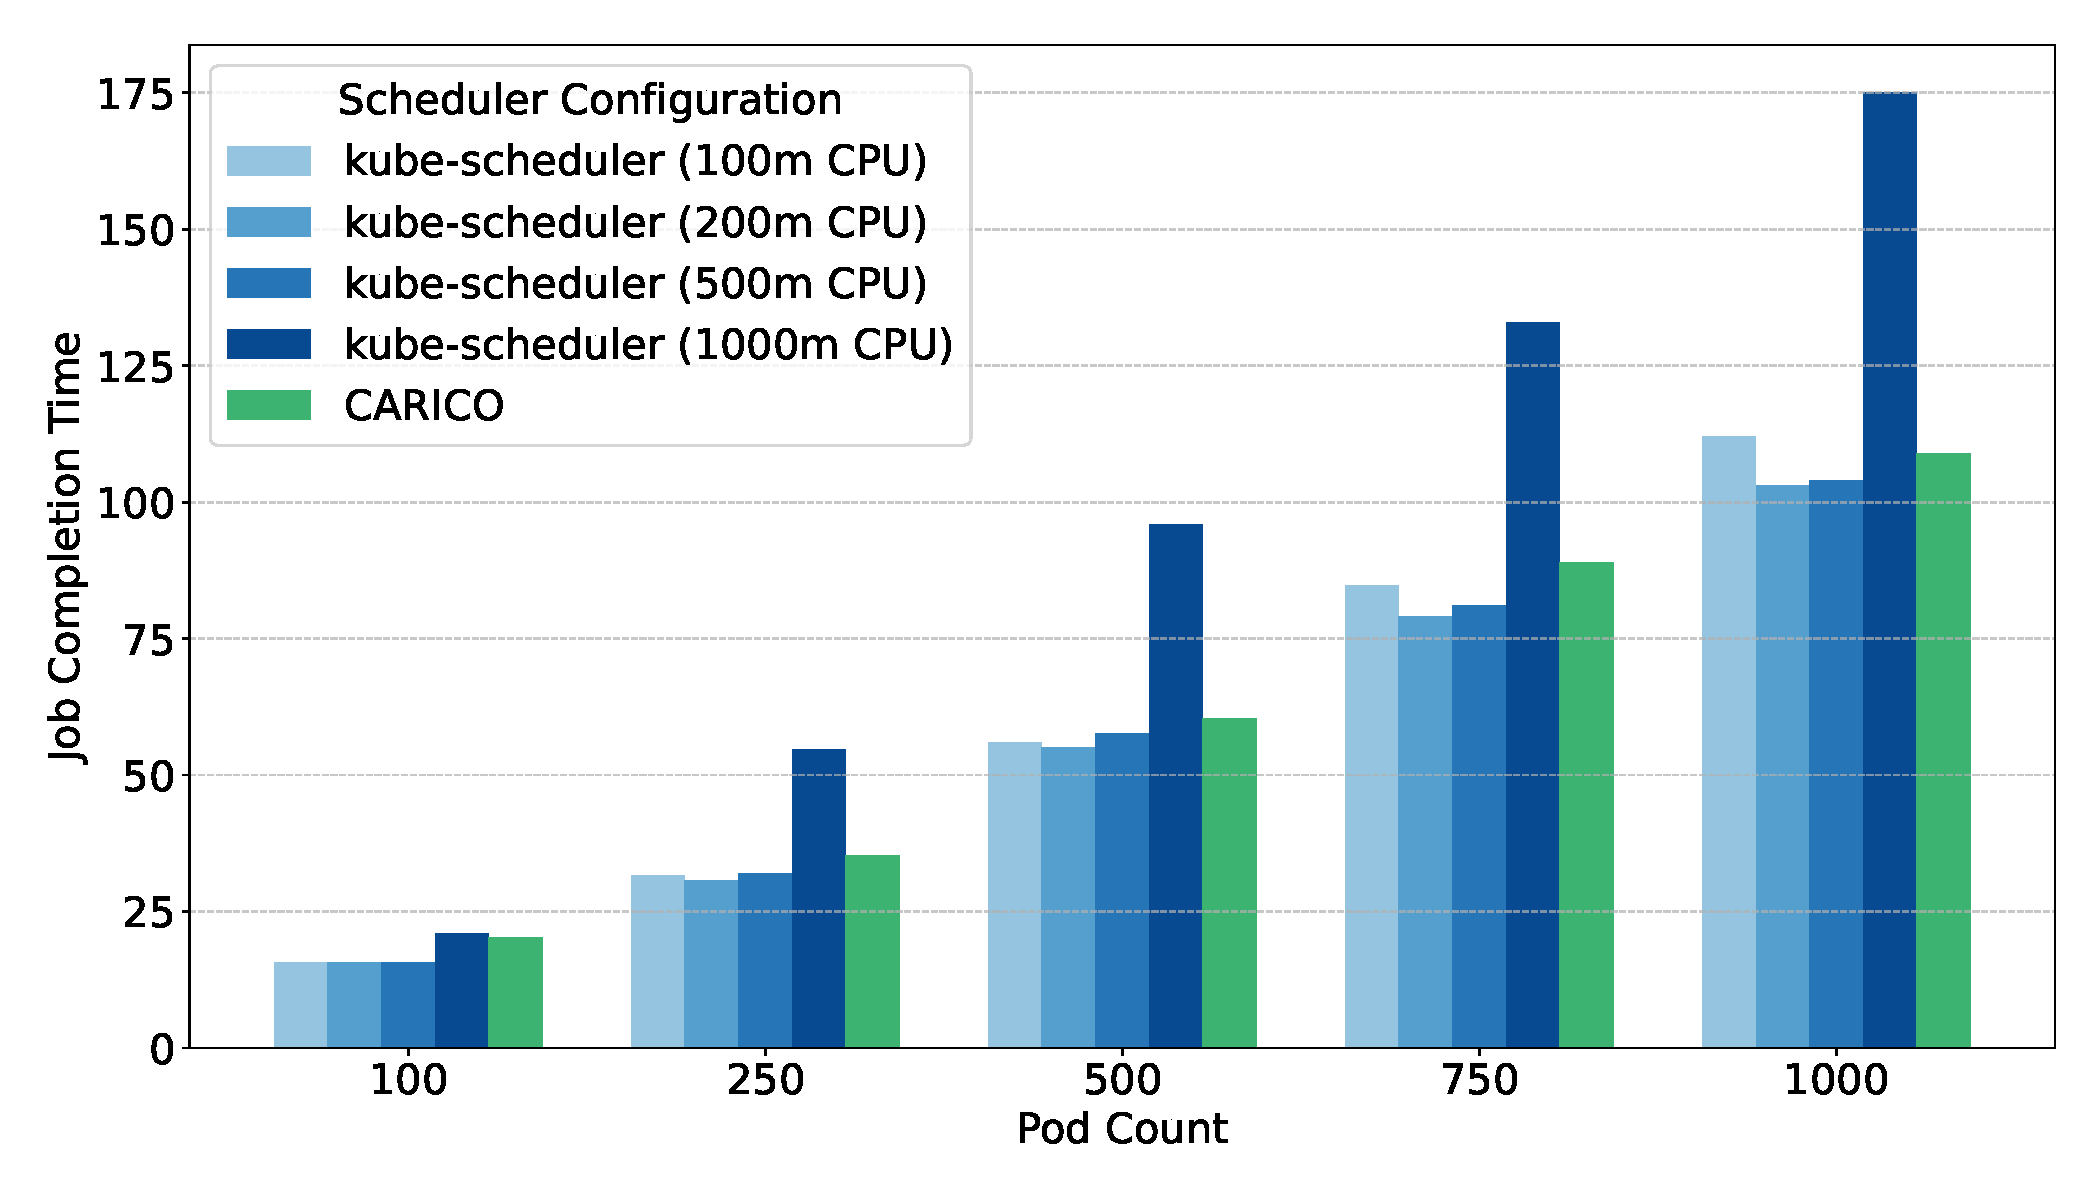
\includegraphics[width=\textwidth]{images/pi-job-completion.pdf}
    \caption{The Job completion of \texttt{pi-2000} Jobs with different Pod
    counts. The requested resources are given when using \texttt{kube-scheduler}}
    \label{fig:pi-2000-throughput}
\end{figure}

Figure \ref{fig:pi-2000-throughput} demonstrates the Job completion of
\texttt{pi-2000} with different Pod counts. We can observe that \textsc{Carico}
is able to consistently achieve comparable Job completions (within $\approx$
10\% of the optimal run with \texttt{kube-scheduler}) without any prior
knowledge of a Pod's resource usage. On the other hand, incorrect Pod requests
can result in $\approx$ 80\% increase in Job completion when using
\texttt{kube-scheduler}.

% \begin{table}[ht!]
% \centering
    % \begin{tabular}{|l|r|r|c|c|}
    % \hline
    % \textbf{Scheduler} & \multicolumn{2}{c|}{\textbf{Requested}} &
        % \multicolumn{2}{c|}{\textbf{Job Completion (s)}} \\ \cline{2-5}
    % &  \textbf{CPU} & \textbf{Memory} & \textbf{100 Pods} & \textbf{200 Pods} \\
    % \hline
        % Default & 200m & 750Mi & 144.3 $\pm$ 0.6 & 362 $\pm$ 20.4\\
        % \textsc{Carico} &  &  & 189 $\pm$ 4.36 & 353.3 $\pm$ 12.7 \\
    % \hline
    % \end{tabular}
    % \caption{Job Completion of Job deployments with different Pod counts. Each
    % Pod executed a small ML workload. For the default scheduler, the requested
    % resources are also given}
    % \label{tab:ml-throughput}
% \end{table}

\begin{figure}[ht!]
    \centering
    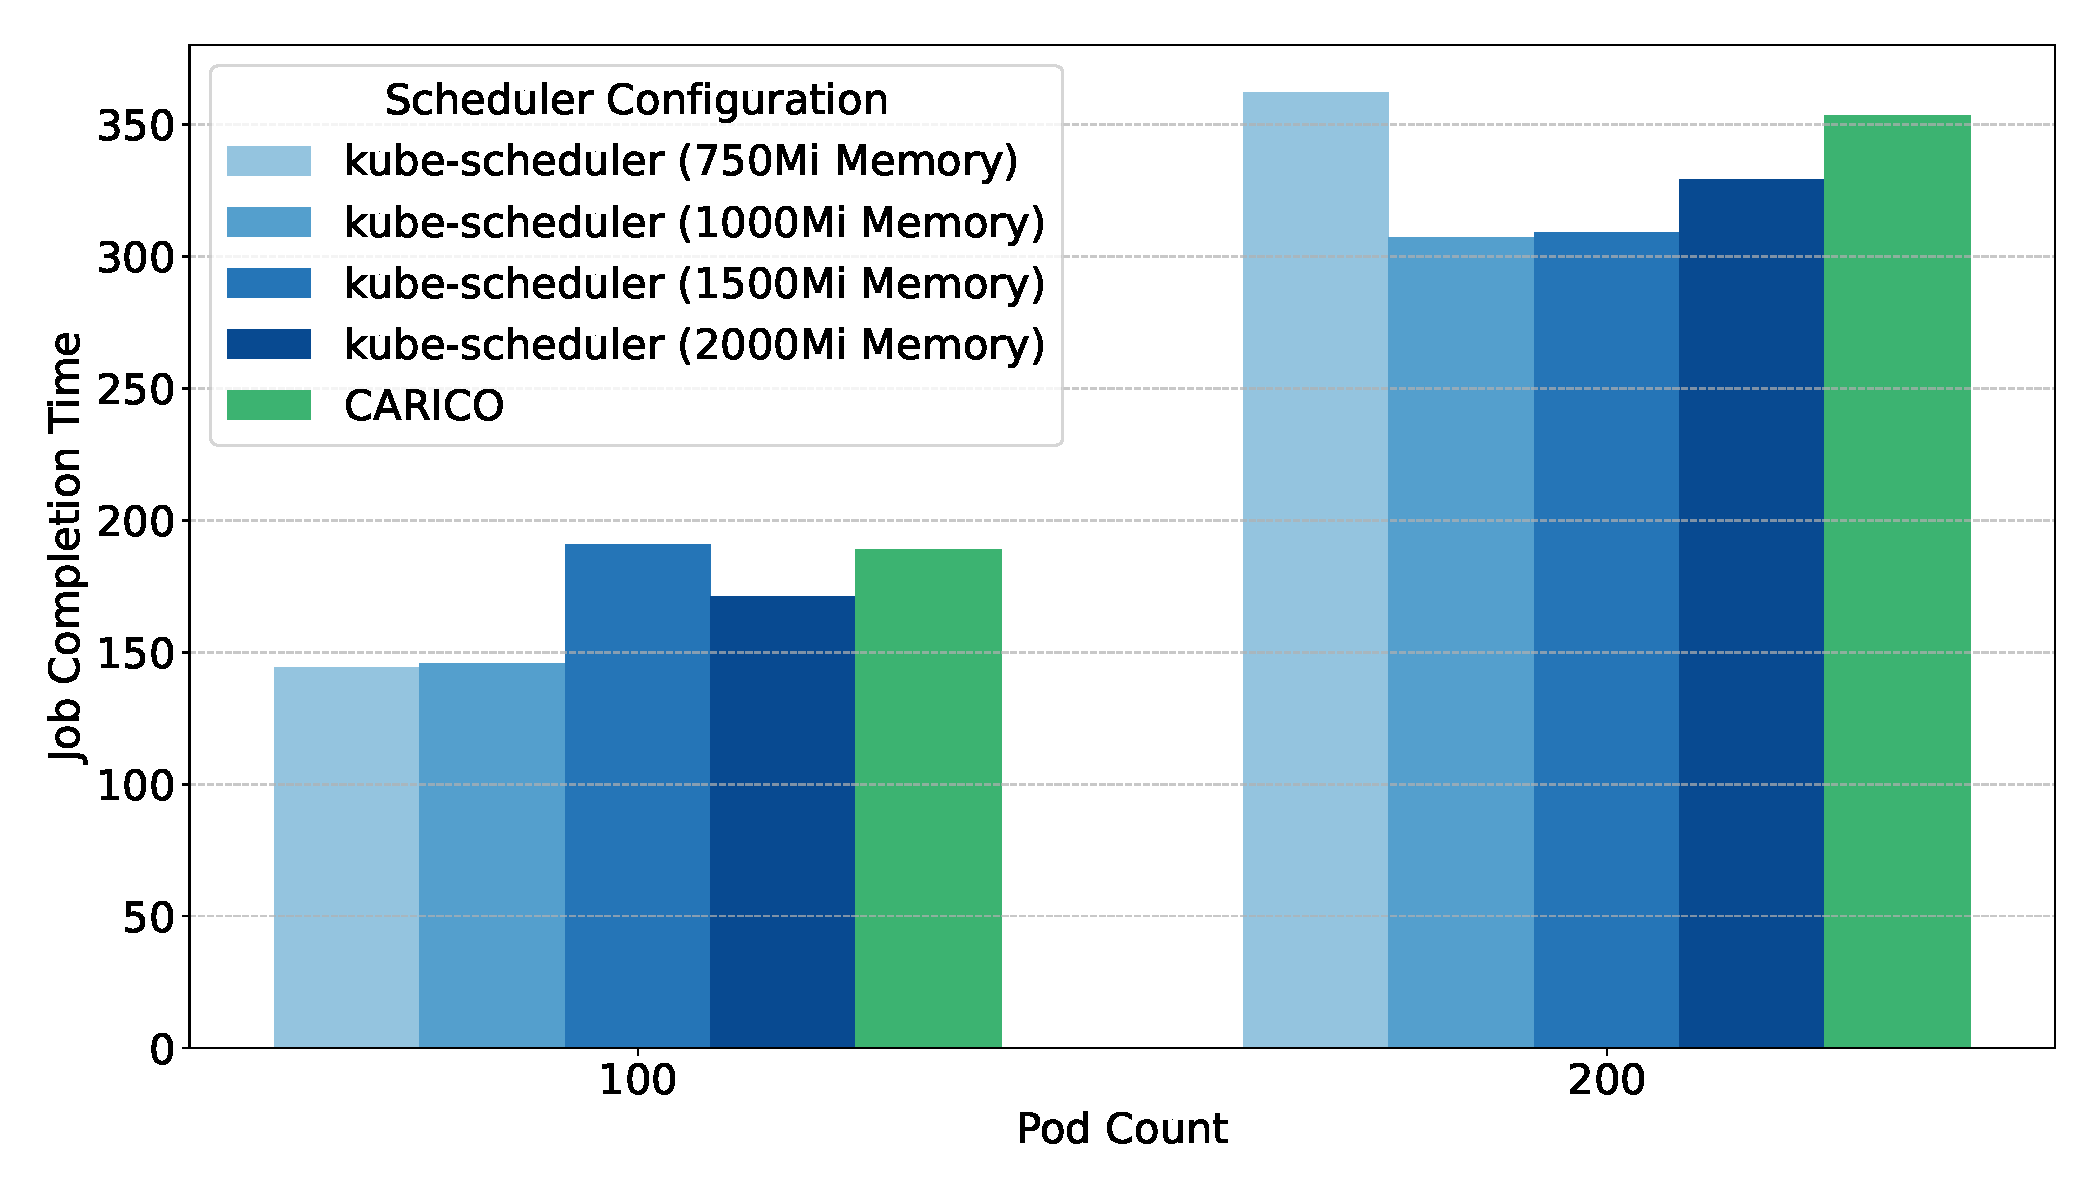
\includegraphics[width=\textwidth]{images/ml-job-completion.pdf}
    \caption{The Job completion of \texttt{sklearn} Jobs with different Pod
    counts. The requested resources are given when using
    \texttt{kube-scheduler}}
    \label{fig:ml-throughput}
\end{figure}

Figure \ref{fig:ml-throughput} presents the Job completion of \texttt{sklearn}
Jobs. Like in Figure \ref{fig:pi-2000-throughput}, \textsc{Carico} is able to
achieves comparable Job completion times using only telemetric data. Similarly,
we can also observe the effect of inaccurate resource requests. More importantly,
underestimating memory usage can result in Nodes running out of memory and
their kernel OOM killing actively running Pods. This often results in Jobs
unable to complete and is the reason for why I do not present Job completions
for runs requesting less than 750Mi bytes of memory.

\section{Pod Completion}
\label{sec:eval-pod-completion}
In this section, I compare the individual Pod Completion times from the traces
of different Job executions.

\begin{table}[h!]
\centering
    \begin{tabular}{|l|r|c|c|c|c|c|c|c|}
    \hline
        \bfseries Scheduler & \bfseries CPU Request & \bfseries Mean & \bfseries Std. &
        \bfseries Min. & \bfseries 25\% & \bfseries Median & \bfseries 75\% & \bfseries Max. \\
    \hline
        Default & 100m & 47.43 & 14.59 & 7.00 & 39.00 & 52.00 & 57.00 & 73.00
        \\
        Default & 500m & 9.55 & 1.49 & 5.00 & 9.00 & 10.00 & 10.00 & 14.00
        \\
        \textsc{Carico} & & 7.69 & 0.99 & 5.00 & 7.00 & 8.00 & 8.00 & 11.00 \\
    \hline
    \end{tabular}
    \caption{Pod Completion of a trace when executing a \texttt{pi-2000} Job
    with 1000 Pods under different schedulers.}
    \label{tab:cpu-pod-completions}
\end{table}

Table \ref{tab:cpu-pod-completions} presents the Pod completion distribution of
the traces from running a 1000 Pod \texttt{pi-2000} Job under different
schedulers. \textsc{Carico} is able to consistently achieve a tight Pod
completion distribution with 75\% of Pods completing in less than 8 seconds. In
contrast, when underestimating resource requests and using 100 milliCPU, the
distribution of Pod completion times becomes tail-heavy with 50\% of Pods taking
longer than 52 seconds to complete and a maximum completion time of 73 seconds.
However, even when using the optimal and more conservative resource request of
500 milliCPU, its distribution has a 25\% higher mean with 50\% more variance.

\begin{figure}[ht!]
    \centering
    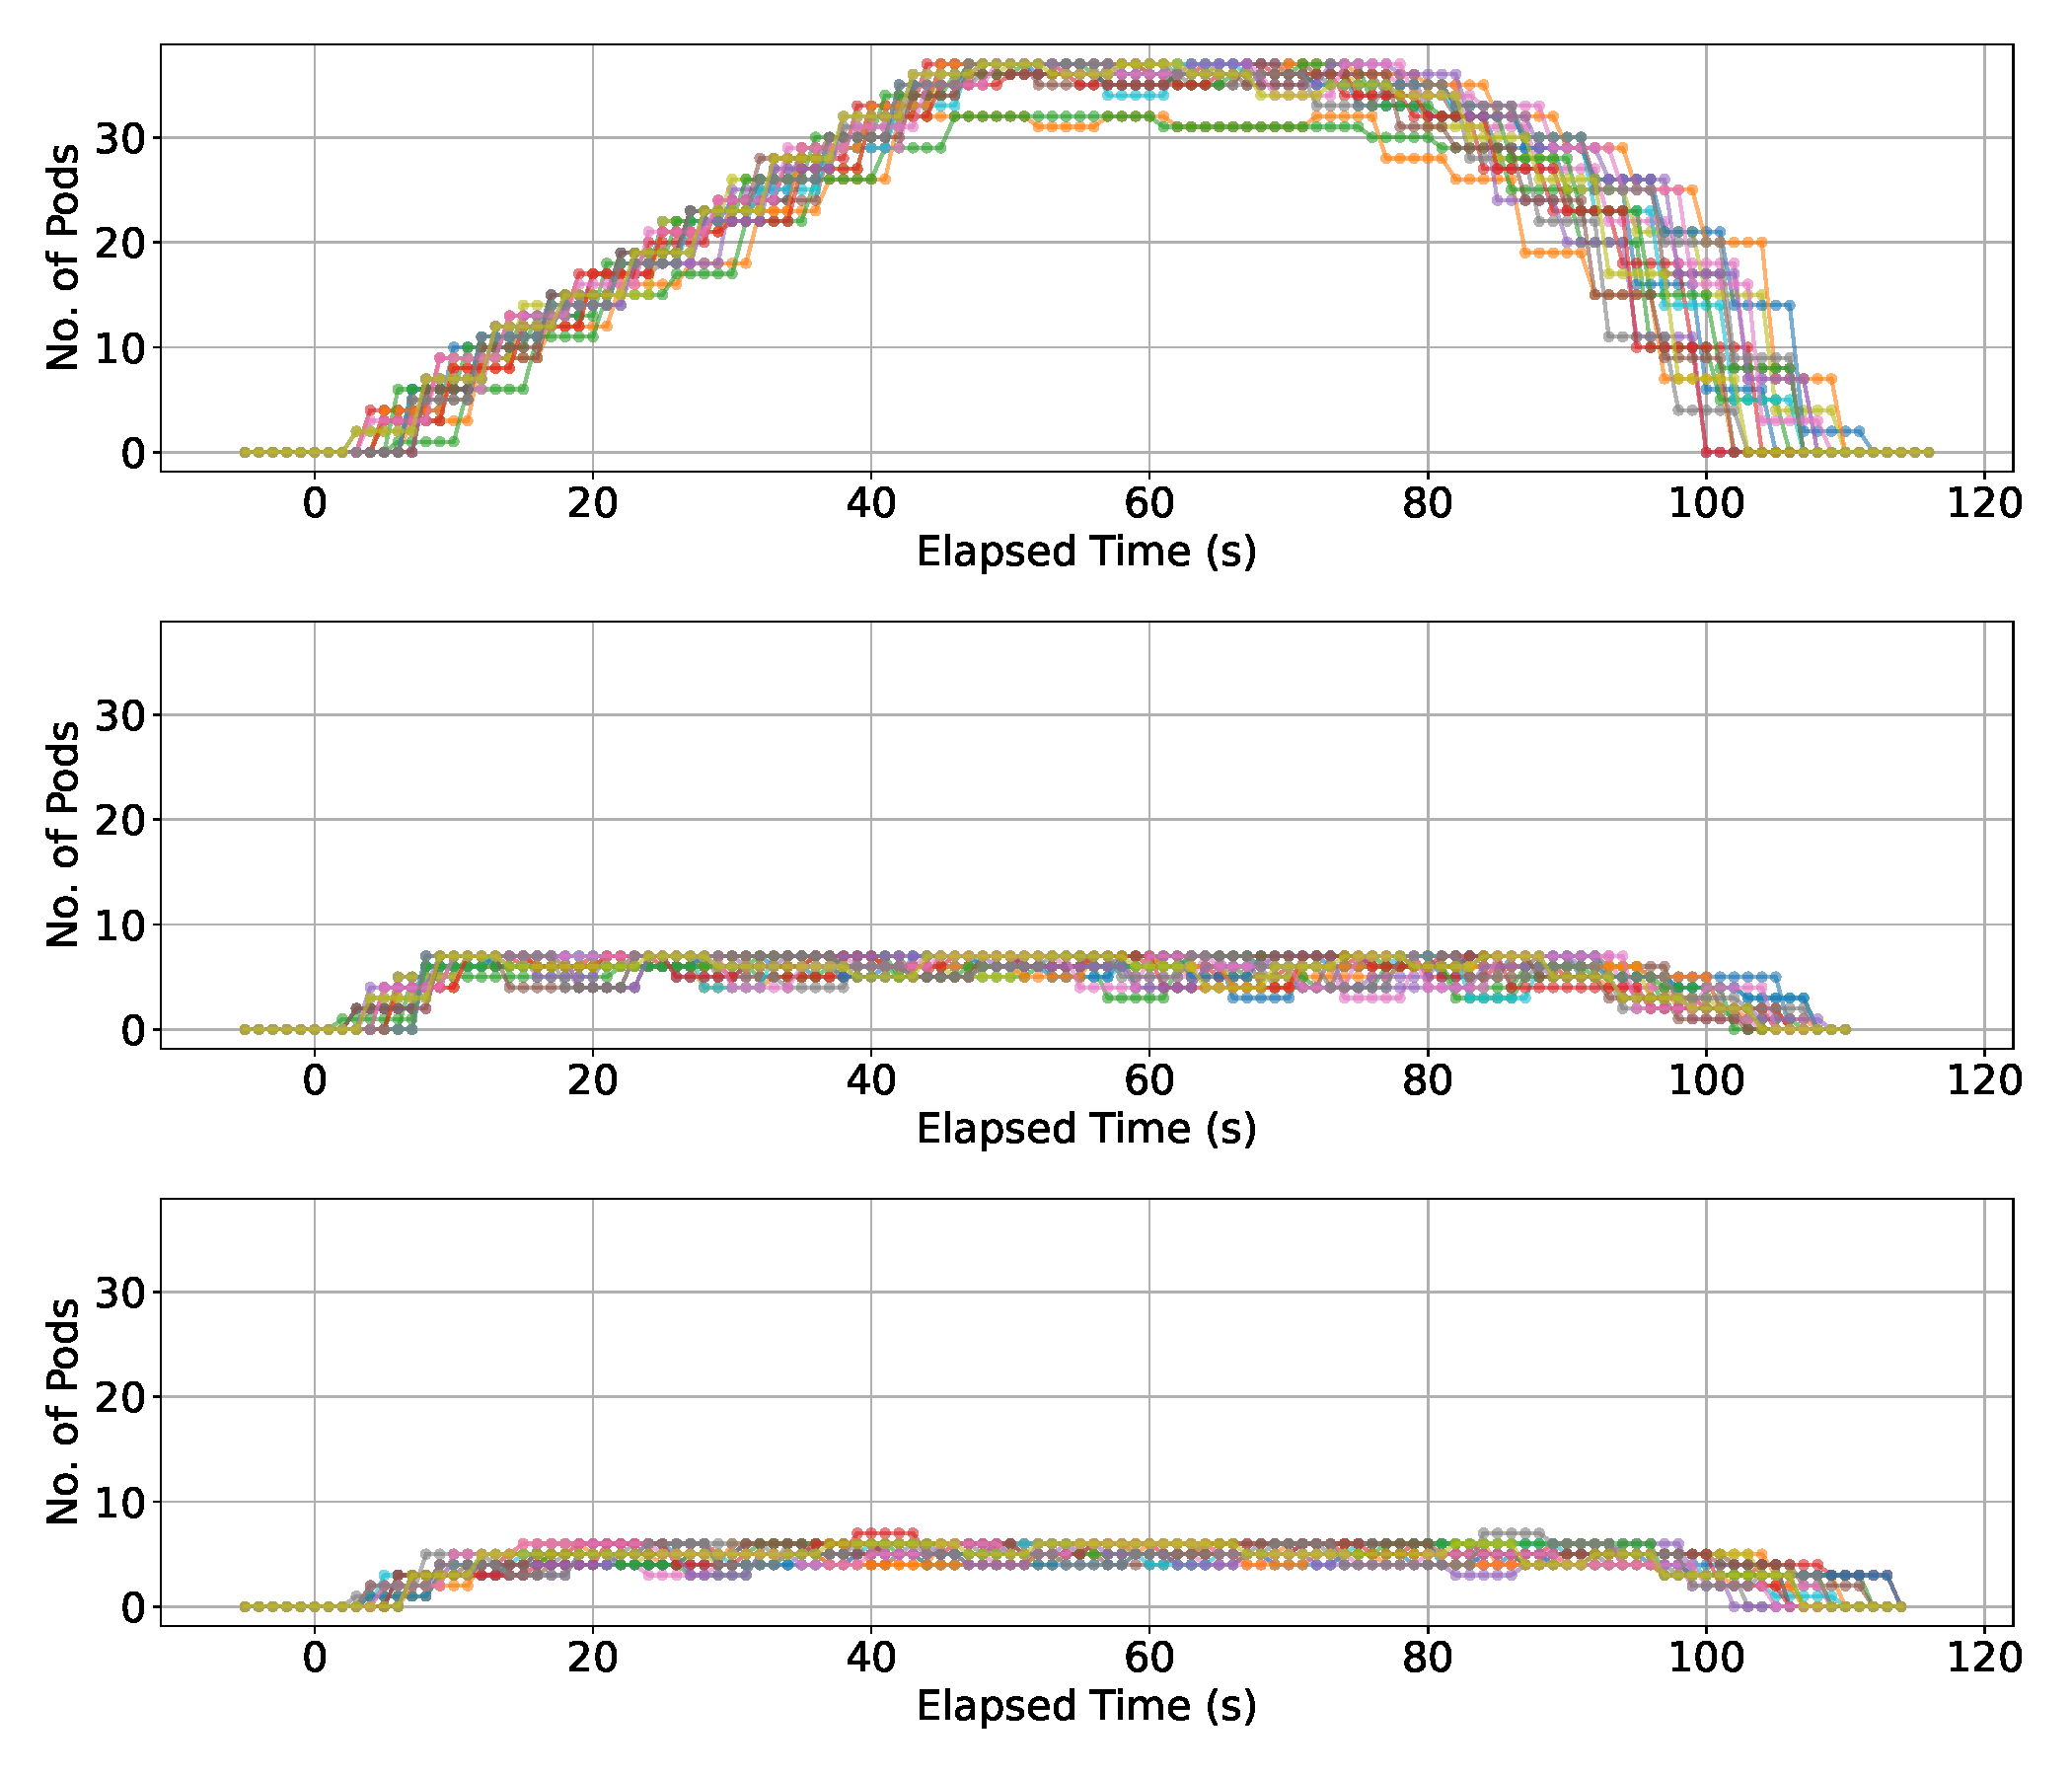
\includegraphics[width=\textwidth]{images/pi-running-pods.pdf}
    \caption{The number of \texttt{pi-2000} Pods running on a Node during the
    execution of a Job with 1000 Pods.}
    \label{fig:pi-2000-1000x-pod-running}
\end{figure}

To further justify the results seen in Table \ref{tab:cpu-pod-completions}, I
plot the number of concurrently running Pods on each Node during the Job traces
in Figure \ref{fig:pi-2000-1000x-pod-running}. When underestimating the resource
request, \texttt{kube-scheduler} is able to pack more Pods on a Node at once.
This results in higher resource contention as more Pods have to share their time
on the CPU. With less time on the CPU per second, Pods take longer to finish
their computation. On the other hand, the more conservative requests means the
\texttt{kube-scheduler} is able to pack fewer Pods, meaning each Pod gets a
reasonable share of time on the CPU and therefore can complete faster. With
\textsc{Carico}, Nodes detect the CPU is at capacity once there is always at
least one process waiting for a CPU core. This therefore limits the number of
Pods a Node can take and ensures all Pods receive an adequate amount of CPU
resources.

\begin{table}[ht!]
\centering
    \begin{tabular}{|l|r|c|c|c|c|c|c|c|}
    \hline
        \bfseries Scheduler & \bfseries \# Pods & \bfseries Mean & \bfseries Std. &
        \bfseries Min. & \bfseries 25\% & \bfseries Median & \bfseries 75\% & \bfseries Max. \\
    \hline
        % Default & 100 & 127.38 & 5.29 & 118 & 123.00 & 126.00 & 132.00 &
        % 138.00 \\
        % \textsc{Carico} & 100 & 59.02 & 14.62 & 27.00 & 55.00 & 61.00 & 66.00 & 94.00 \\
        Default & 200 & 225.19 & 36.19 & 45.00 & 231.00 & 236.00 & 239.00 &
        244.00\\
        \textsc{Carico} & 200 & 64.46 & 14.33 & 23.00 & 57.75 & 67.00 & 73.25 & 89.00 \\
    \hline
    \end{tabular}
    \caption{Pod Completion of a trace when executing a \texttt{sklearn} Job
    with 200 Pods under different schedulers.}
    \label{tab:mem-pod-completions}
\end{table}

Table \ref{tab:mem-pod-completions} presents the Pod completion distribution of
the traces from running a 200 Pod \texttt{sklearn} Job under different
schedulers. \textsc{Carico} is still able to consistently achieve a tight Pod
completion distribution with a mean completion time of 64.46 seconds and a
variance of 14.33 seconds.  On the other hand, when using the lowest
overestimate of memory utilisation, 750Mi bytes of memory,
\texttt{kube-scheduler} achieves a $3.5 \times$ higher mean Pod completion time
with more than twice the variance.

\begin{figure}[ht!]
    \centering
    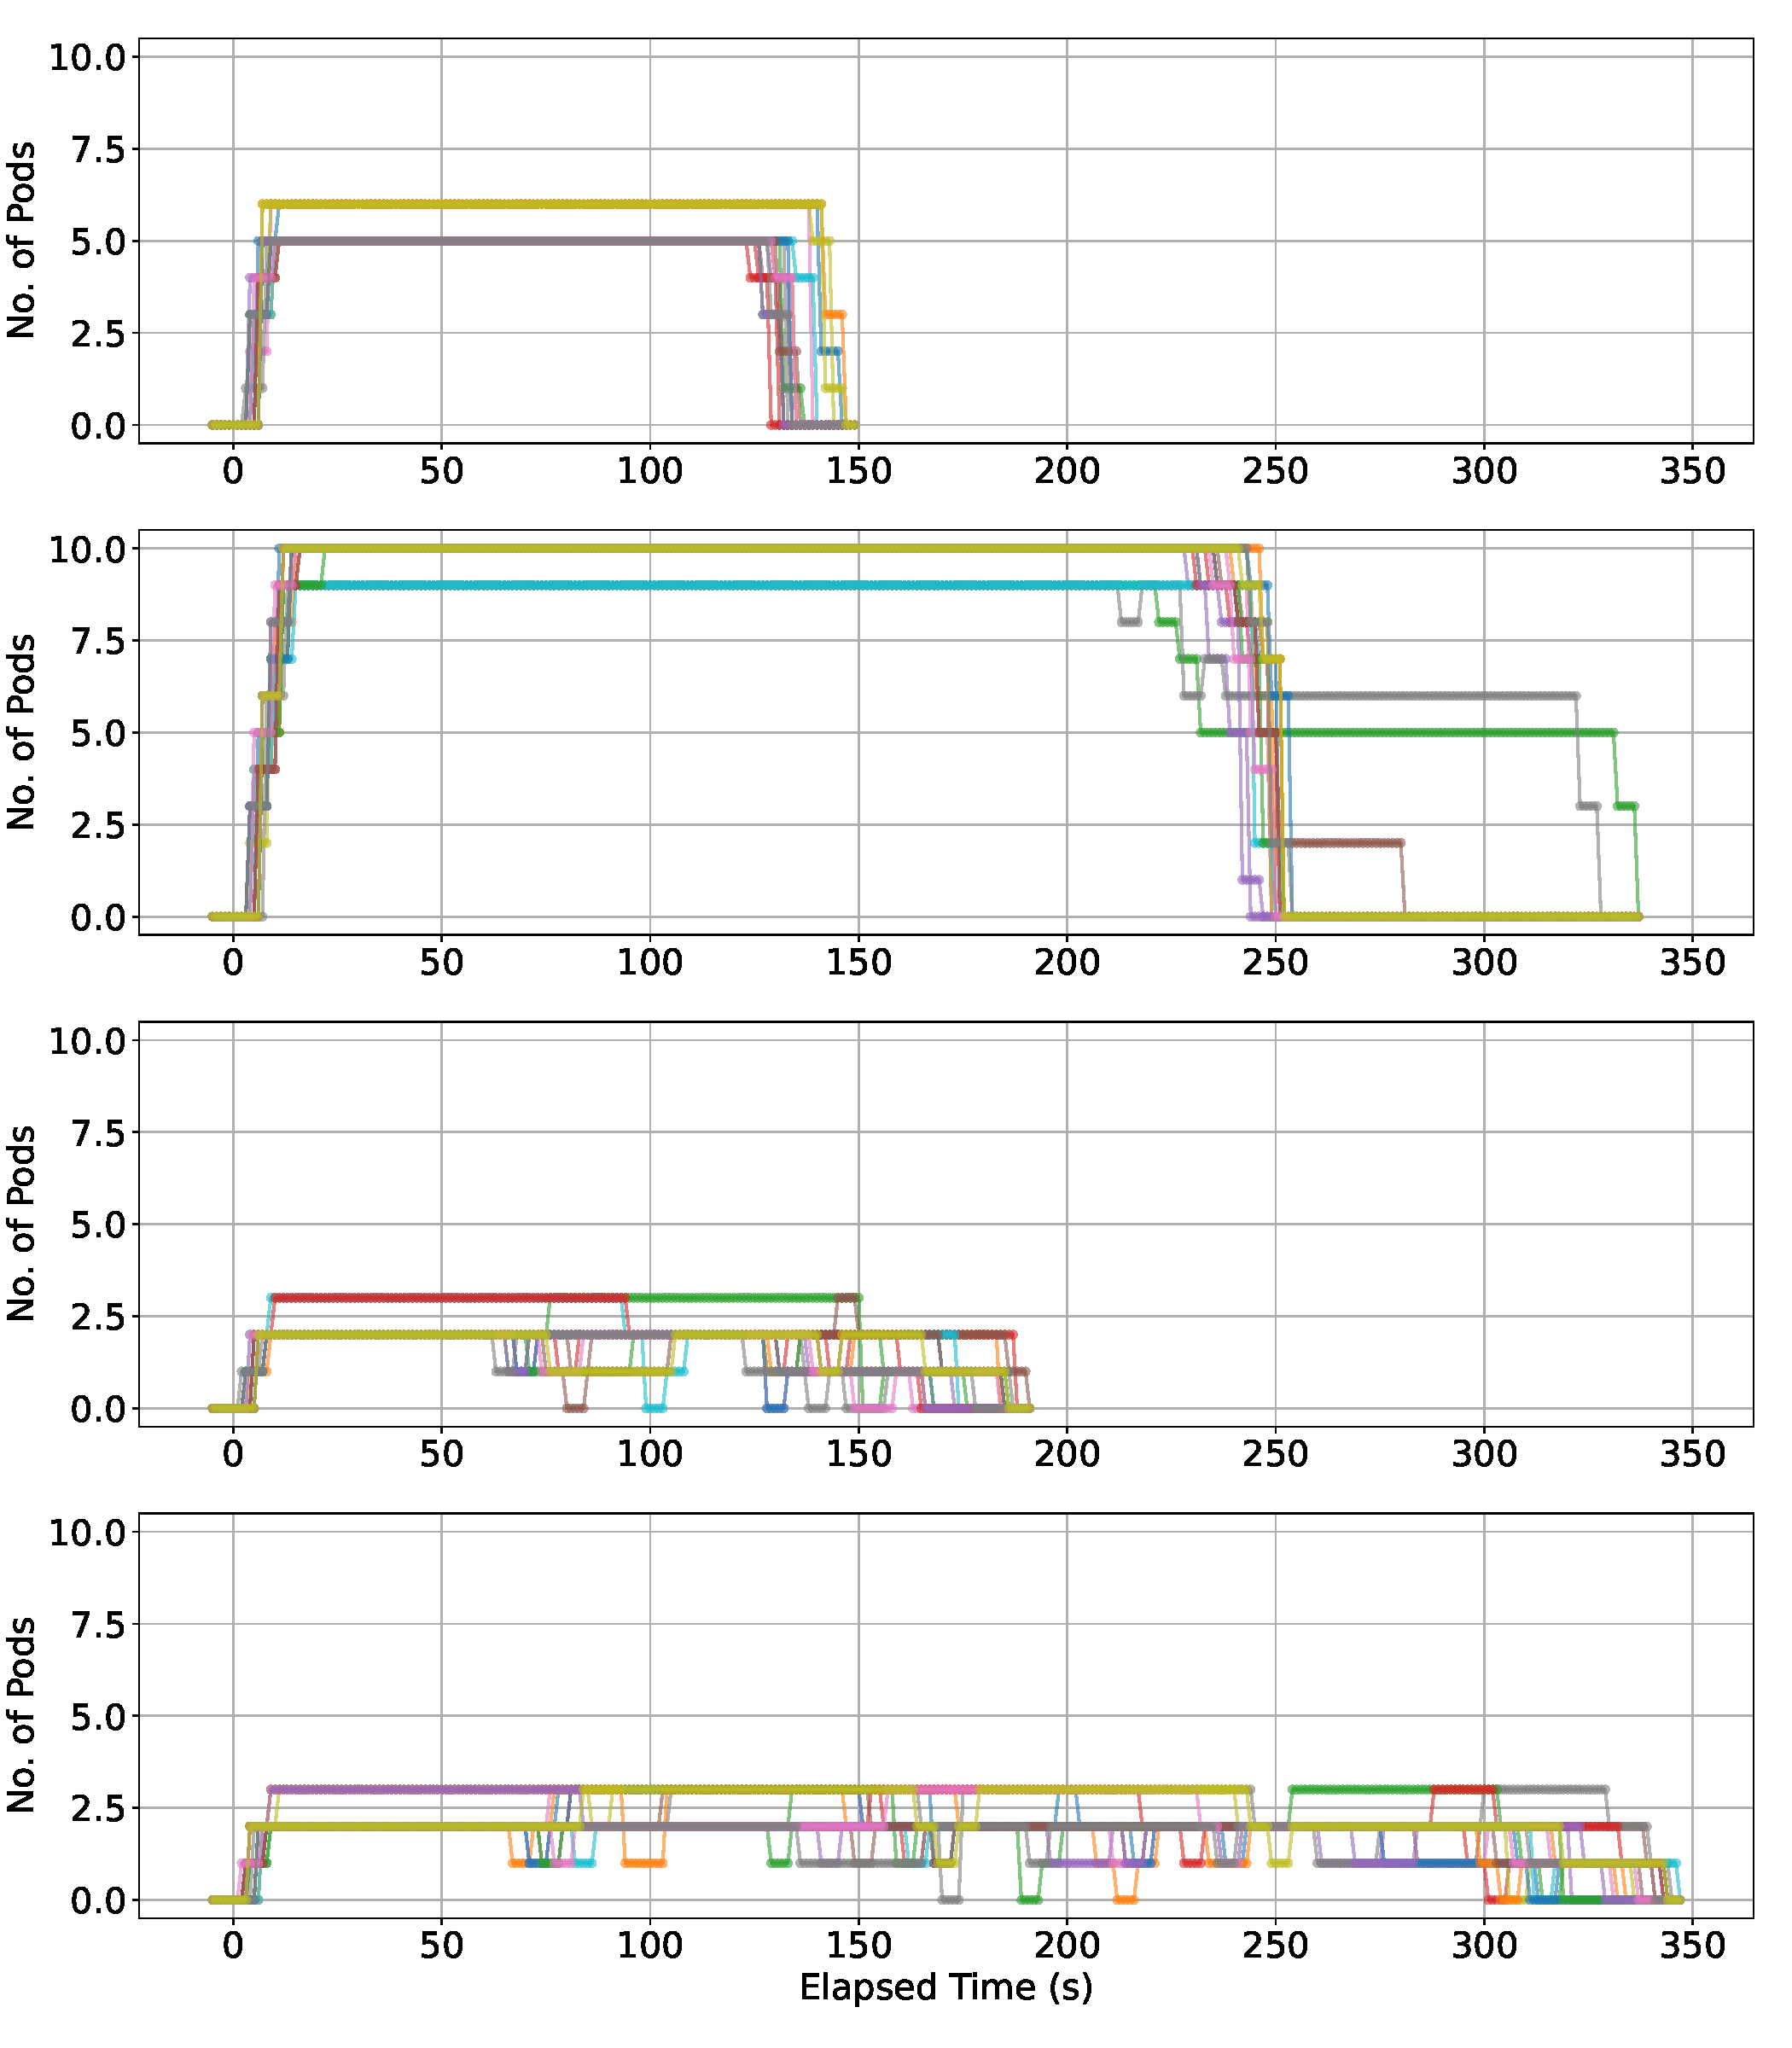
\includegraphics[width=\textwidth]{images/ml-running-pods.pdf}
    \caption{The number of \texttt{sklearn} Pods running on a Node during the
    execution of a 200 Pods Job.}
    \label{fig:ml-pod-running}
\end{figure}

Like with \texttt{pi-2000}, \texttt{kube-scheduler} allocates more Pods onto a
Node at once, resulting in higher resource contention, and thus longer Pod
completion times. This graph also explains the longer Job completion time. Due
to the memory request (750 Mi) and each Node's capacity (8GB),
\texttt{kube-scheduler} is unable to allocate all the Pods in one sweep.
However, once the Pods on the faster machines (imbalance caused by the
hypervisor) complete, \texttt{kube-scheduler}'s greedy nature causes it to
allocate all the remaining Pods to those machines. The long running time of the
\texttt{sklearn} Pods combined with the resource contention from allocating the
remaining Pods to a small number of machines means the Job must wait longer for
the last Pod to complete. On the other hand, \textsc{Carico} ensures a
consistent number of Pods are running on a Node.

\section{Resource Utilisation}
\label{sec:eval-util}
In this section, I investigate the resource utilisation during the Job traces
explored in Section \ref{sec:eval-pod-completion}.

\begin{figure}[h]
    \centering
    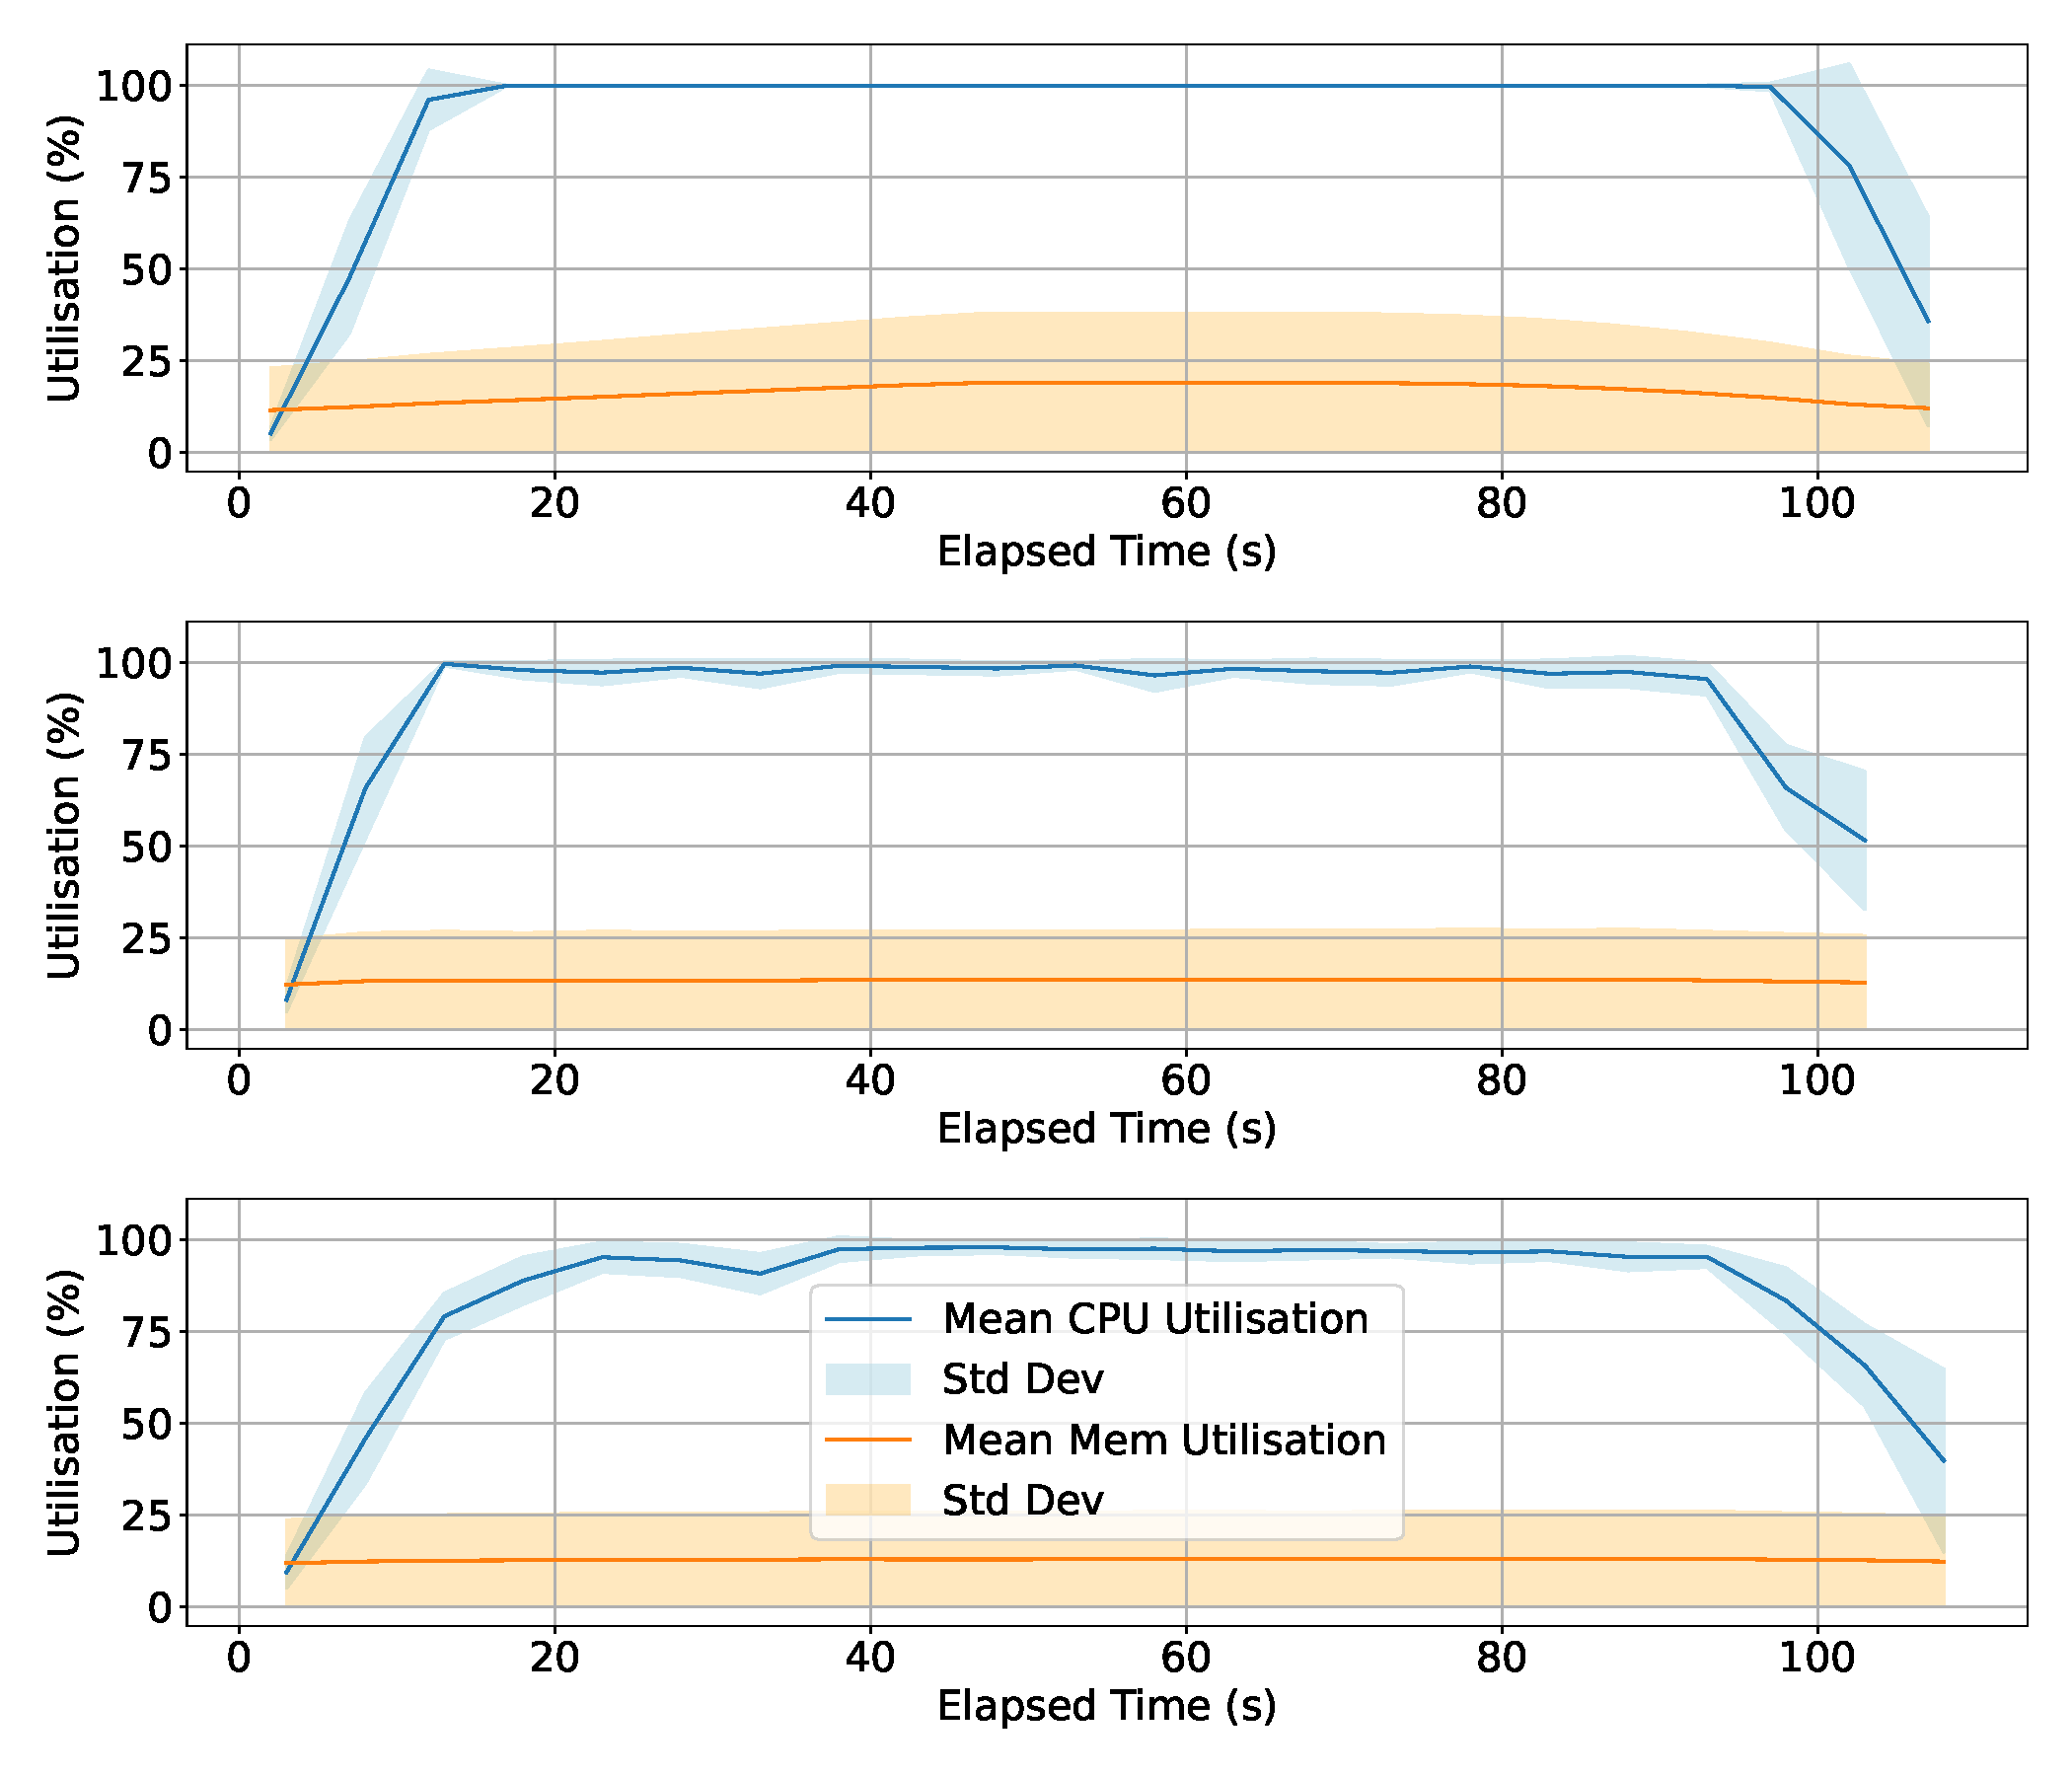
\includegraphics[width=\textwidth]{images/pi-util.pdf}
    \caption{Resource utilisation during a trace of executing a \texttt{pi-2000}
    Job with 1000 Pods under different schedulers.}
    \label{fig:pi-2000-1000x-pod-util}
\end{figure}

Figure \ref{fig:pi-2000-1000x-pod-util} illustrates the resource utilisation
during the execution of a 1000 \texttt{pi-2000} (CPU-focused) Pod Job. When
under-estimating the resource request, \texttt{kube-scheduler} is able to easily
maximise the CPU utilisation, with all Nodes reading 100\% CPU utilisation. The
more conservative 500 milliCPU request is still able to achieve close to 100\%
CPU utilisation. Although, \textsc{Carico} takes a more than twice as long to
reach $\geq 95$\%, it achieves consistently high CPU utilisation.

\begin{figure}[ht!]
    \centering
    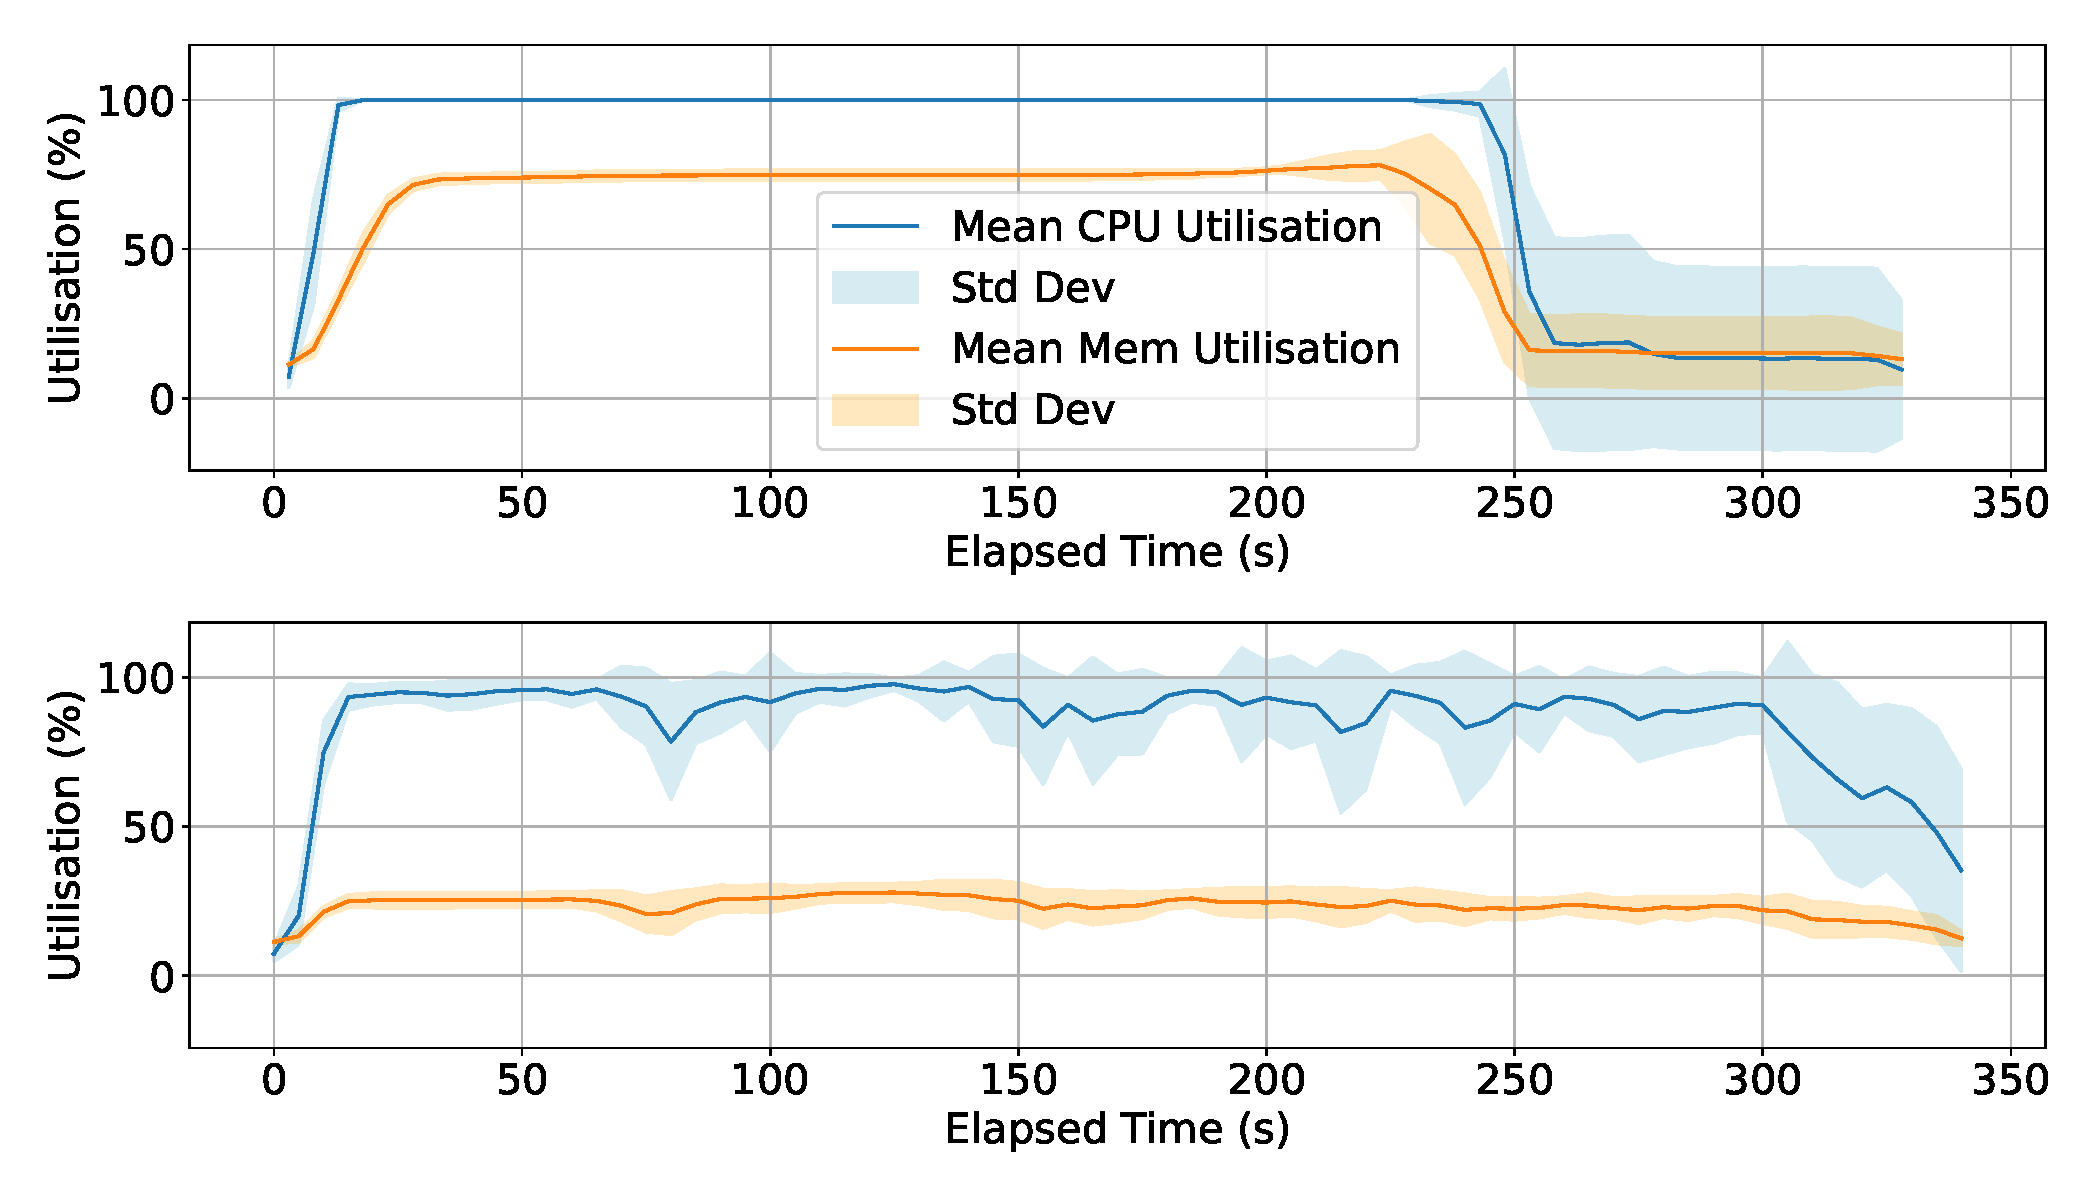
\includegraphics[width=\textwidth]{images/ml-util.pdf}
    \caption{Resource utilisation during a trace of executing a \texttt{sklearn}
    Job with 200 Pods under different schedulers.}
    \label{fig:ml-util}
\end{figure}

Figure \ref{fig:ml-util} presents the resource utilisation during the execution
of a 200 \texttt{sklearn} (memory-focused) Pod Job. While \textsc{Carico} again
achieves high CPU utilisation, it fails to fully utilise memory. This indicates
that even with \texttt{sklearn}'s significantly large memory footprint, CPU
still became the bottleneck resource. As a result, Nodes would limit capacity
before fully utilising memory. Contrastingly, as \textsc{kube-scheduler} does
not use live-telemetry, it is able to pack enough \texttt{sklearn} pods to
achieve a higher memory utilisation. However, this trace also highlights
problems caused by \texttt{kube-scheduler}'s greedy bin-packing.
Figure~\ref{fig:ml-pod-running} from Section~\ref{sec:eval-pod-completion}
painted the scenario in which \texttt{kube-scheduler} results in a mostly idle
cluster waiting for a small number of machines to finish executing the remaining
Pods. We can observe this impact on resource utilisation, as during the last
minute of the Job's execution, the clusters average CPU and memory utilisation
is around $\approx 10$\%.

\section{Workload Heterogeneity}
\label{sec:eval-hetero}
To investigate how \textsc{Carico} handles workloads with different
characteristics, I executed both the \texttt{pi-2000} and \texttt{sklearn} Jobs.
\texttt{pi-2000} Pods requests 100 milliCPUs, while \texttt{sklearn} Pods
requested 200 milliCPUs and 750Mi of memory.

\textbf{Throughput}\\
\begin{figure}[ht!]
    \centering
    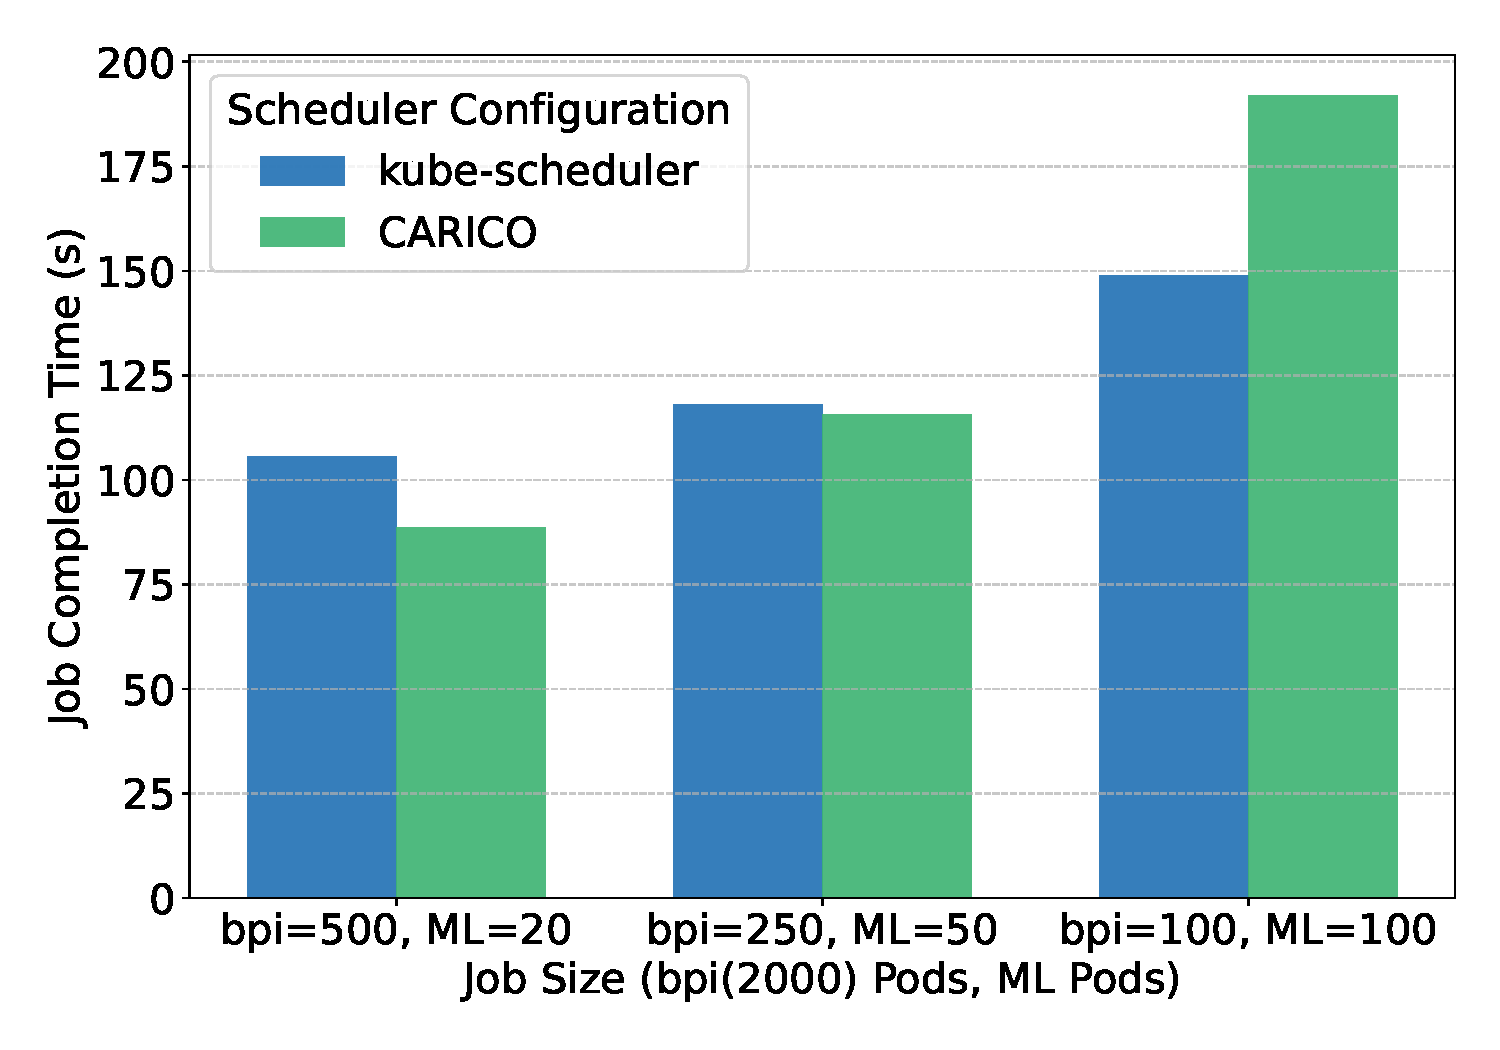
\includegraphics[width=\textwidth]{images/mixed-job-completion.pdf}
    \caption{Job Completion of multi-resource Job deployments with different Pod
    counts. For the default scheduler, \texttt{bpi(2000)} Pods requested 100
    milliseconds of CPU and ML Pods requested 200 milliseconds CPU and 750Mi of
    memory}
    \label{fig:mixed-throughput}
\end{figure}

Figure \ref{fig:mixed-throughput} presents the Job Completion time when running
\texttt{pi-2000} and \texttt{sklearn} Jobs with varying distributions.
\textsc{Carico} is able to achieve lower Job completion times when executing a
larger portion of \texttt{pi-2000}. However, once a significant portion of the
workloads are long-running \texttt{sklearn} Pods, \texttt{kube-scheduler} edges
ahead. This is likely because the interference from \texttt{pi-2000} Pods are
small enough where the performance resembles that of running only
\texttt{sklearn} Pods.

% \begin{table}[ht!]
% \centering
    % \begin{tabular}{|l|c|c|c|}
    % \hline
    % \textbf{Scheduler} & \multicolumn{2}{c|}{\textbf{Job Size}} &
        % \textbf{Job Completion (s)} \\ \cline{2-3}
        % &  \texttt{bpi(2000)} & \texttt{ML} & \\
    % \hline
        % Default & 500 & 20 & 105.7 $\pm$ 10.6 \\
        % \textsc{Carico} & 500 & 20 & 88.7 $\pm$ 2.5 \\
        % Default & 250 & 50 & 118 $\pm$ 4.58 \\
        % \textsc{Carico} & 250 & 50 & 115.7 $\pm$ 0.58 \\
        % Default & 100 & 100 & 149 $\pm$ 0.0 \\
        % \textsc{Carico} & 100 & 100 & 192 $\pm$ 4.0 \\
    % \hline
    % \end{tabular}
    % \caption{Job Completion of multi-resource Job deployments with different Pod
    % counts. For the default scheduler, \texttt{bpi(2000)} Pods requested 100
    % milliseconds of CPU and ML Pods requested 200 milliseconds CPU and 750Mi of
    % memory}
    % \label{tab:mixed-throughput}
% \end{table}

\textbf{Pod Completions}\\
\begin{table}[ht!]
\centering
    \begin{tabular}{|l|c|c|c|c|c|c|c|c|}
    \hline
        \bfseries Scheduler & \bfseries Job & \bfseries Mean & \bfseries Std. &
        \bfseries Min. & \bfseries 25\% & \bfseries Median & \bfseries 75\% & \bfseries Max. \\
    \hline
        Default & \texttt{pi-2000} & 28.78 & 7.52 & 7.00 & 27.00 & 30.00 & 33.00 & 45.00 \\
        Default & \texttt{sklearn} & 65.25 & 10.53 & 49.00 & 58.25 & 64.00 & 75.25 & 82.00 \\
        \textsc{Carico} & \texttt{pi-2000} & 7.40 & 1.14 & 5.00 & 7.00 & 7.00 & 8.00 & 11.0 \\
        \textsc{Carico} & \texttt{sklearn} & 34.50 & 7.39 & 22.00 & 27.50 & 36.00 & 40.25 & 44.00 \\
    \hline
    \end{tabular}
    \caption{Pod Completion of a trace when concurrently executing a 500 Pod \texttt{pi-2000}
    Job and a 20 Pod \texttt{sklearn} Job.}
    \label{tab:mixed-pod-completions}
\end{table}

I also investigated how Pod Completion time changes when running diverse
workloads. Table \ref{tab:mixed-pod-completions} presents the distributions of
the Pod Completion for both \texttt{pi-2000} and \texttt{sklearn} Jobs. From it
we can see how \textsc{Carico} continues to achieve significantly lower mean Pod
Completion times with both Jobs than \texttt{kube-scheduler}. Furthermore, the
achieved Pod Completion times vary significantly less with \textsc{Carico}
($\approx 7 \times$ lower) than those of \texttt{kube-scheduler}.
% TODO: SHOULD I ONLY INVESTIGATE WORKLOADS WE HAVE SEEN BEFORE SO THAT I CAN
% COMPARE THE CHANGE IN DISTRIBUTION

\begin{figure}[ht!]
    \centering
    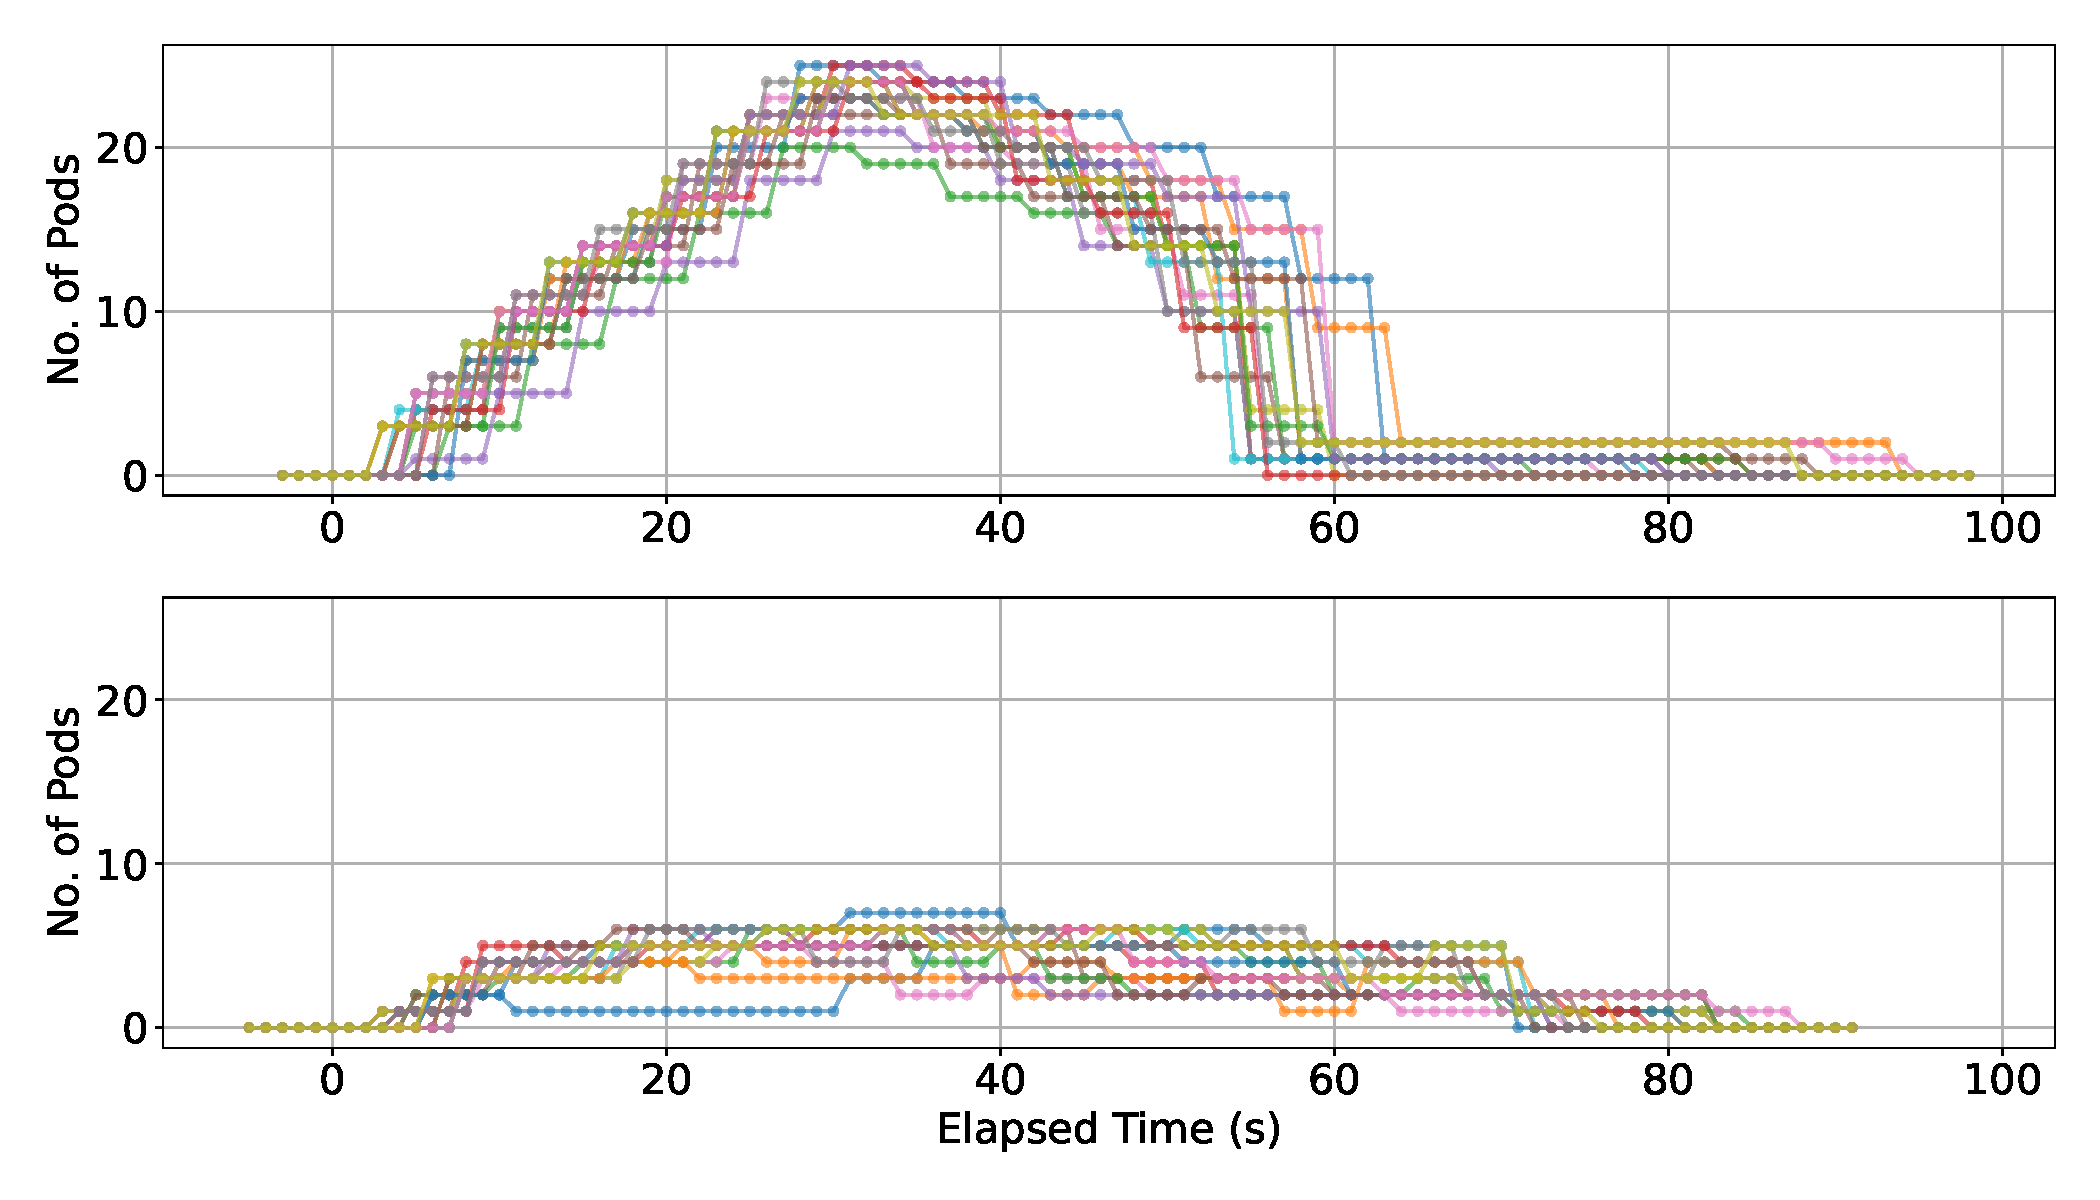
\includegraphics[width=\textwidth]{images/mixed-running-pods.pdf}
    \caption{The number of Pods running on a Node when executing concurrently a
    500 Pod \texttt{pi-2000} Job and a 20 Pod \texttt{sklearn} Job.}
    \label{fig:mixed-pod-running}
\end{figure}

Further investigation into the number of Pods running on each Node, depicted in
Figure \ref{fig:mixed-pod-running}, shows how \textsc{Carico} achieves a
consistent number of running Pods throughout the job, while with
\texttt{kube-scheduler} the number of running Pods varied from 25 Pods to less
than 3 Pods.

\textbf{Resource Utilisation}\\
\begin{figure}[ht!]
    \centering
    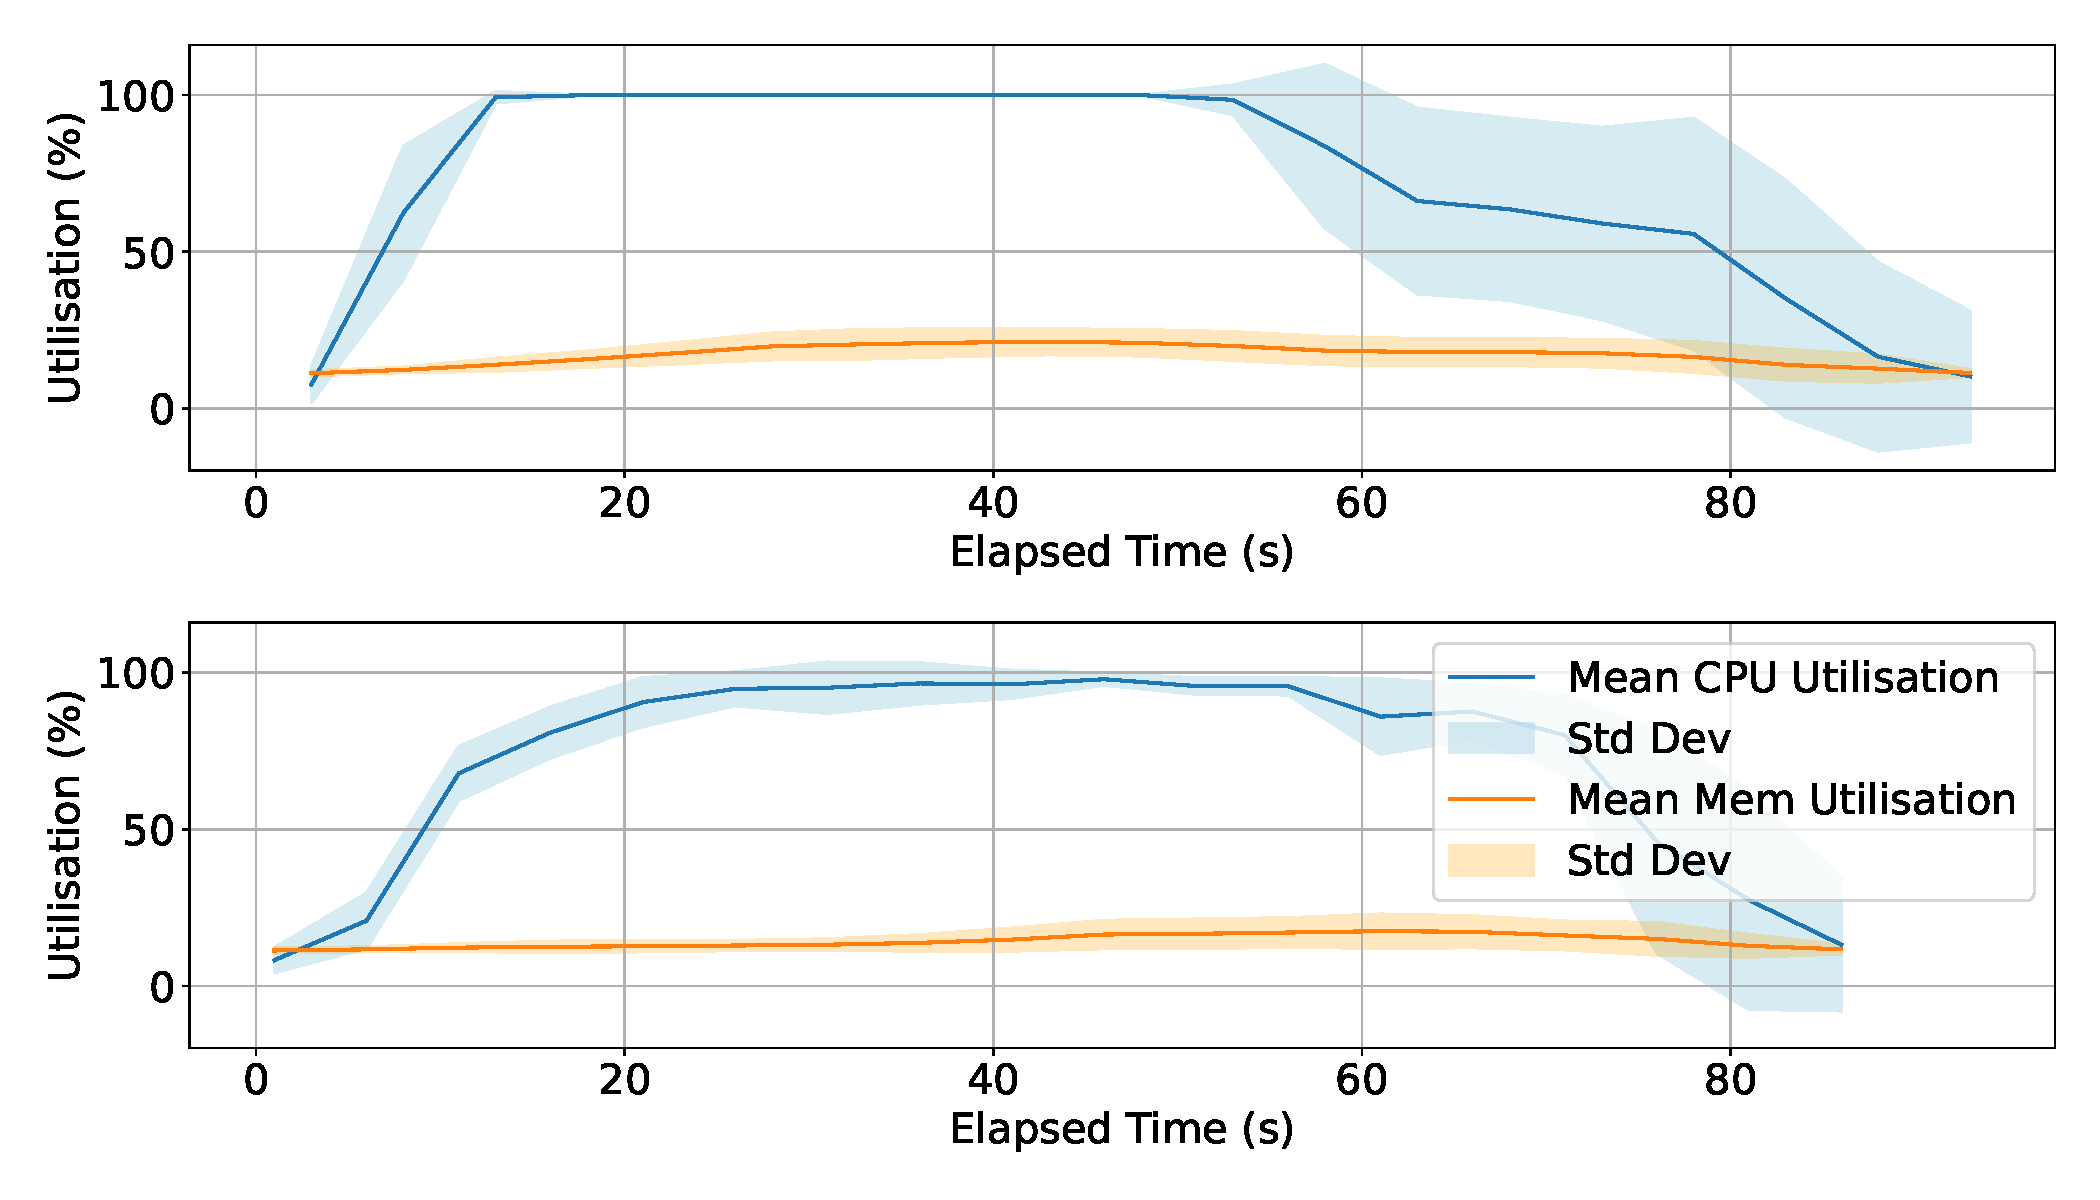
\includegraphics[width=\textwidth]{images/mixed-util.pdf}
    \caption{Resource utilisation during a trace of executing concurrently a 500
    Pod \texttt{pi-2000} Job and a 20 Pod \texttt{sklearn} Job.}
    \label{fig:mixed-util}
\end{figure}

Figure \ref{fig:mixed-util} shows the resource utilisation when executing a 500
Pod \texttt{pi-2000} Job and a 20 Pod \text{sklearn} Job concurrently. We can
see the impact of \texttt{kube-scheduler}'s varying number of Pods running on
each Node. When Nodes have more than 20 Pods running on them, they advertise
100\% CPU utilisation, which is indicative of high resource contention. Then,
when only a few \texttt{sklearn} Pods remain on a Node, the overall mean CPU
utilisation of the clusterdrops to less than 75\%. In constrast, \textsc{Carico}
achieves a high CPU utilisation $\geq 95$\% without experiencing extreme
contention. Furthermore, its balanced allocation ensures a high CPU utilisation
throughout the entire execution time of the Jobs.

\section{Workload Isolation}
\label{sec:eval-isolation}
To evaluate \textsc{Carico}'s QoS, I investigated how its scheduling decisions impact the
performance of already running Pods. For this experiment, I had a Pod running on
a worker Node, while another Pod periodically sent HTTP GET requests. This
polling Pod would then measure latency of the response. I then scheduled a Job
of 1000 Pods executing \texttt{bpi(2000)} across the cluster and measured how
the response latency changed. In the default schedulers case, each Pod requested
100 milliseconds of CPU time.

\begin{table}[h!]
\centering
    \begin{tabular}{|l|c|c|c|c|c|c|}
    \hline
    \textbf{Scenario} & \multicolumn{6}{c|}{\textbf{Response Latency (ms)}} \\
    \cline{2-7}
    & \textbf{Min} & \textbf{Med} & \textbf{P90} & \textbf{P95} & \textbf{P99} & \textbf{Max} \\
    \hline
    Baseline & 0.99 & 3.04 & 3.78 & 4.00 & 4.47 & 8.32 \\
    Default Scheduler & 1.07 & 10.06 & 18.61 & 22.28 & 28.82 & 54.49\\
    \textsc{Carico}  & 1.00 & 2.48 & 6.09 & 7.82 & 10.53 & 17.39\\
    \hline
    \end{tabular}
    \caption{The distribution of a servers response latency when different
    schedulers attempt to allocate a 1000 Pod Job across the server.}
    \label{tab:impacted-latency}
\end{table}

Table \ref{tab:impacted-latency} contains the measured distribution of the
response latency from the server. It shows how scheduling with the default
scheduler using 100m CPU requests, resulting a significant shift in latency
distribution. The median more than doubles and the distribution greatly shifted
towards the tail: the maximum latency was $\approx \times7$ larger. On the other
hand, when scheduling with \textsc{Carico}, the median latency actually decreased.
Furthermore, while the tail distribution did increase, the max latency was only
$\approx \times2$ bigger.

\section{\textsc{Carico} Overhead}
\label{sec:eval-overhead}
To measure the overhead incurred from running the \textsc{Carico} pods on the Nodes, I
compared the completion time of Jobs when running on Nodes with and without the
\textsc{Carico} deployment. I considered easuring resource utilisation on a Node with
just the \textsc{Carico} Pod running, but much of the behaviour of the
\textsc{Carico} Pod occurs during container events. As a result, the measured overhead
would not represent the entire impact of the \textsc{Carico} Pod. Instead, by measuring
the overhead over Jobs, we aggregate the impact of \textsc{Carico} across multiple
container events, providing a more holistic view of its impact.

\begin{table}[ht!]
\centering
    \begin{tabular}{|c|c|}
    \hline
    \textbf{Number of Pods} & \textbf{\% Overhead with \textsc{Carico}} \\
    \hline
        100 & -2.33 $\pm$ 3.29 \\
        250 & -1.19 $\pm$ 2.44 \\
        500 & 4.84  $\pm$ 1.25 \\
        750 & 1.69  $\pm$ 0.42 \\
        1000 & 2.27  $\pm$ 0.66 \\
    \hline
    \end{tabular}
    \label{tab:overhead}
    \caption{The overhead incurred when running \textsc{Carico} Pods on Nodes during the
    executing of Jobs with varying Pod counts. Each Pod executed
    \texttt{bpi(2000)} and requested 200 milliseconds of CPU time.}
\end{table}

To measure \textsc{Carico}'s overhead, I used Pod's executing \texttt{bpi(2000)}. Table
\ref{tab:overhead} presents the relative change in Job Completion time with
\textsc{Carico} Pods running on the Nodes. We can see that the Job Completion time of
smaller Jobs are more noisy, therefore, resulting in an observed decrease in Job
Completion times. However, with larger and more stable Jobs, the overhead from
\textsc{Carico} is more visible. From these observations we can conclude that \textsc{Carico} has
$\approx$ 2\% overhead.

\section{Limitations}

Firstly, \textsc{Carico} is a telemetry-based scheduler and thus relies on accurate
telemetry that is able to accurately capture a Node's true limit, after which
over-contention results in degraded performance. During this dissertation, we
have observed how this is not guaranteed. VMs, like those I used in my
evaluation, only have access to a simulated hardware provided by the underlying
hypervisor. As a result, symptoms of over-contention, such as the overhead from
CPU or cache thrashing, are not observed when a VM reports high CPU utilisation.
This supported by Figure \ref{fig:podcount-util-pressure}: the Job Completion
time per Pod when executing a Job on a single Node, continued to decrease even
after the Node reported full CPU pressure. Consequently, \textsc{Carico}
allocates fewer Pods to Nodes reducing Job completion.

Secondly, \textsc{Carico} can only learn about Pod workloads once they have
already been scheduled and observed. This can limit performance, as
\textsc{Carico} is unable to discern new Pods with potentially complementary directions
of resource usage from those it has already observed. Conversely, a
high-intensity workload may be submitted after a low-intensity one, and
\textsc{Carico}'s recent low Per-Pod-Cost estimate could result in a over-eager
Nodes accepting too many high-intensity workloads before \textsc{Carico} has
time to detect the new resource usage. This situation could then cause
performance degradation or even the termination of Pods. \textsc{Carico}
attempts to mitigate this by having the Per-Pod-Cost slowly increase when there
are no Pods running, however, this has a limited impact for workloads that
arrive in quick succession.
